\documentclass[aspectratio=169]{beamer}
\usepackage[T1]{fontenc}
\usepackage{lmodern}
\usepackage{hyperref}

% other packages
\usepackage{latexsym,amsmath,xcolor,multicol,booktabs,calligra}
\usepackage{graphicx}
\graphicspath{{pic/}{../figures/}}
\renewcommand{\figurename}{Figure.}
\renewcommand{\tablename}{Table.}

\author{Kelompok 2}
\title{Analisis Kestabilan dan Bifurkasi Model Oregonator \\ dari Reaksi Kimia Belousov–Zhabotinsky}
\subtitle{\textit{Mini Project} Sistem Dinamik}
%\institute{Departemen Matematika \\ Universitas Gadjah Mada}
\date{Juni 2024 \\ \footnotesize Versi terkoreksi, Oktober 2026}
\usepackage{sisu}

\begin{document}

\begin{frame}
    \titlepage
    \begin{figure}[htpb]
        \begin{center}      
\includegraphics[width=0.15\linewidth]{logo_ugm.jpg}
        \end{center}
    \end{figure}
\end{frame}

\begin{frame}{Kelompok 2}
    Anggota Kelompok:\\
    \begin{tabular}{cll}
        &1. & Nimas Roro Ayuningsih\\
        &2. & Vincentius Stanisluiz Ferrel\\
        &3. & Chatarina Hana Febriyanti\\
        &4. & Kasih Bijaksana Karunia Ilahi\\
        &5. & Moh Hasbi Alfarizi
    \end{tabular}
\end{frame}

\begin{frame}{Outline}
    \tableofcontents[
sectionstyle=show,subsectionstyle=show/shaded/hide,subsubsectionstyle=show/shaded/hide]
\end{frame}

\section{Pendahuluan}

\subsection{Model Oregonator}

\begin{frame}{Model Oregonator}
    \textbf{Persamaan Reaksi Belousov - Zhabotinsky} diberikan sebagai berikut.
    \begin{align*}
        \begin{array}{lllll}
            (R3) & BrO^-_3 + Br^- + 2H^+ \to HBrO_2 + HOBr\\
            (R2) & HBrO_2 + Br^- + H^+ \to 2HOBr\\
            (G) & 2Ce^{3+} + BrO^-_3 + HBrO_2 + 3H^+ \to 2Ce^{4+} +     2HBrO_2 + H_2 O\\
            (R4) & 2HBrO_2 \to BrO^-_3 + HOBr + H^+\\
            (R10) & 4Ce^{4+} + BrMA + 2H_2 O \to 4Ce^{3+} + HCOOH + 2CO_2 + 5H^+
        \end{array}
    \end{align*}
    Selanjutnya, dimisalkan
    \begin{align*}
        X = [HBrO_2] ;\ Y = [Br^-] ;\ Z = [Ce^{4+}] ;\ A = [BrO^-_3] ;\ B = [BrMA] ;\ P = [HOBr]
    \end{align*}
\end{frame}

\begin{frame}{Model Oregonator}
    Menggunakan Oregonator Scheme, diperoleh
    \begin{align*}
        A+Y &\to X + P, & v &= k_3 AY\\
        X + Y &\to 2P, & v &= k_2 XY\\
        A + X &\to 2X + 2Z, & v &= k_5 AX\\
        2X &\to A + P, & v &= k_4 X^2\\
        B + Z &\to fY, & v &= k_0 BZ
    \end{align*}
    dengan
    \begin{align*}
        k_0 = 0.4/MS; \ k_2 = 2 \times 10^9/MS; \ k_3 = 2/MS; \ k_4 = 4 \times 10^7/MS; \ k_5 = 10^4/MS
    \end{align*}
\end{frame}

\begin{frame}{Model Oregonator}
    Selanjutnya, dengan hukum laju reaksi "The Law of Mass Action", diperoleh \textbf{sistem dinamik} berupa laju perubahan X,Y,Z sebagai berikut.
    \begin{align*}
        \frac{dX}{dt} &= k_3 AY - k_2 XY + k_5 AX - 2k_4 X^2\\
        \frac{dY}{dt} &= -k_3 AY - k_2 XY + fk_0 BZ\\
        \frac{dZ}{dt} &= 2k_5 AX - k_0 BZ
    \end{align*}
\end{frame}

\subsection{Model Matematika}

\begin{frame}{Model Matematika}
    Sistem dinamik yang telah diperoleh dapat disederhanakan menjadi bentuk non dimensional. Dimisalkan
    \begin{align*}
        x = \frac{X}{X_0}; \ y = \frac{Y}{Y_0}; \ z= \frac{Z}{Z_0}; \ \tau = \frac{t}{T_0}
    \end{align*}
    dengan
    \begin{align*}
        X_0 = \frac{k_5 A}{2k_4}; \ Y_0 = \frac{k_5 A}{k_2}; \ Z_0 = \frac{(k_5 A)^2}{k_4 k_0 B}; \ T_0 = \frac{1}{k_0 B}
    \end{align*}
\end{frame}

\begin{frame}{Model Matematika}
    Diperoleh persamaan sistem yang lebih sederhana
    \begin{align*}
        \frac{dx}{d\tau} &= \frac{1}{\epsilon} (qy - xy + x(1-x))\\
        \frac{dy}{d\tau} &= \frac{1}{\delta} (-qy - xy + 2fz)\\
    \frac{dz}{d\tau} &= x-z
    \end{align*}
    dengan
    \begin{align*}
        \epsilon = \frac{k_0 B}{k_5 A}; \ \delta = \frac{2k_0 k_4 B}{k_2 k_5 A}; \ q = \frac{2k_4 k_3}{k_2 k_5}; \ f = \text{parameter stoikiometri}
    \end{align*}
    Dengan konstanta laju di atas, $q = 8 \times 10^{-6}$.
\end{frame}

\section{Pembahasan}

\subsection{Titik Kesetimbangan}

\begin{frame}{Titik Kesetimbangan}
    Akan dicari titik setimbang dari sistem persamaan di atas, yang memenuhi
    \begin{align*}
        \tfrac{dx}{d\tau} = \tfrac{1}{\epsilon} (qy - xy + x(1-x)) = 0, \quad
        \tfrac{dy}{d\tau} = \tfrac{1}{\delta} (-qy - xy + 2fz) = 0, \quad
        \tfrac{dz}{d\tau} = x-z = 0
    \end{align*}
    Dari $z = x$ dan $y = \tfrac{2fx}{q+x}$, titik setimbang taknol memenuhi $x^2 - (1-2f-q)x - q(1+2f) = 0$.
    Diperoleh titik setimbang $E_1^*=(0,0,0)$ dan $E_2^*=(x^*,y^*,z^*)$, di mana
    \begin{align}
        & x^* = z^* = \tfrac{1-2f-q+\sqrt{D}}{2}, \qquad
          y^* = \tfrac{2fx^*}{q+x^*} = \tfrac{2f(1-2f-q+\sqrt{D})}{1-2f+q+\sqrt{D}},  \notag \\
        & D = (1-2f-q)^2 + 4q(1+2f) = 1+q^2+4f^2+2q+12qf-4f > 0. \notag
    \end{align}
    Karena hasil kali kedua akar adalah $-q(1+2f) < 0$, selalu ada tepat satu akar positif,
    sehingga $E_2^*$ ada untuk \textbf{setiap} $f > 0$.
\end{frame}

\subsection{Kestabilan Titik Kesetimbangan}

\begin{frame}{Kestabilan Titik Kesetimbangan}
    Matriks Jacobian sistem adalah
    \begin{align*}
        J = \begin{pmatrix}
            \frac{1-2x-y}{\epsilon} & \frac{q-x}{\epsilon} & 0 \\
            -\frac{y}{\delta} & -\frac{q+x}{\delta} & \frac{2f}{\delta} \\
            1 & 0 & -1
        \end{pmatrix}.
    \end{align*}
    Diperoleh persamaan karakteristik dari Jacobian Matriks di titik $E_1^{*}$
    \begin{equation*}
        \lambda^3 + \left( \tfrac{\epsilon(\delta+q)-\delta}{\epsilon \delta} \right)\lambda^2 + \left( \tfrac{q(\epsilon-1)-\delta}{\epsilon \delta}\right)\lambda-\left( \tfrac{q(2f+1)}{\epsilon \delta}\right)=0
    \end{equation*}
    Suku konstantanya negatif, sehingga polinomial karakteristik bernilai negatif di $\lambda = 0$ dan menuju $+\infty$:
    ada nilai eigen real positif. Jadi titik setimbang $E_1^*=(0,0,0)$ tidak stabil untuk semua parameter.
\end{frame}

\begin{frame}{Kestabilan Titik Kesetimbangan}
    Diperoleh persamaan karakteristik dari Jacobian Matriks di titik $E_2^{*}$
    \begin{equation*}
        \lambda^3 + A\lambda^2 + B\lambda+C=0,
    \end{equation*}
    dengan $a = \tfrac{x^{*2}+q(x^*+2f)}{q+x^*}$ dan
    \begin{align*}
        A &= \tfrac{a}{\epsilon}+\tfrac{q+x^*}{\delta}+1 > 0 \\
        B &= \tfrac{a}{\epsilon}+\tfrac{q+x^*}{\delta}+\tfrac{1}{\epsilon\delta}\left(a(q+x^*)+\tfrac{2fx^*(q-x^*)}{q+x^*} \right) \\
        C &= \tfrac{x^{*2}+q(1+2f)}{\epsilon \delta} > 0
    \end{align*}
    Berdasarkan kriteria kestabilan Routh-Hurwitz, agar sistem stabil, haruslah $AB - C > 0$ dan agar sistem tidak stabil, haruslah $AB - C < 0$.
\end{frame}

\subsection{Analisis Bifurkasi}

\begin{frame}{Analisis Bifurkasi}
    Diperhatikan bahwa pada saat $AB - C = 0 \iff B = \dfrac{C}{A}$, persamaan karakteristik $J_2$ menjadi
\begin{equation*}
    \lambda^3 + A\lambda^2 + \dfrac{C}{A}\lambda + C=0 \iff (\lambda + A)\left(\lambda^2 + \dfrac{C}{A}\right) = 0,
\end{equation*}
yang memiliki akar-akar $\lambda_1 = -A, \lambda_{2,3}=\pm i\sqrt{\frac{C}{A}}$. Akibatnya, $J_2$ memiliki sepasang nilai eigen imajiner murni dan satu nilai eigen real negatif $\lambda_1 = -A$.
Jika pasangan nilai eigen tersebut memotong sumbu imajiner dengan laju taknol
($\tfrac{d}{df}\mathrm{Re}\,\lambda \neq 0$), maka terjadi bifurkasi Hopf.
\end{frame}

\begin{frame}{Analisis Bifurkasi}
    Nilai eigen bergantung pada $\epsilon$, $\delta$, $q$, dan $f$. Dengan $\epsilon$, $\delta$, $q$ tetap,
    $f$ dipilih sebagai parameter bifurkasi.

    \medskip
    Untuk parameter simulasi ($\epsilon = 5\times10^{-5}$, $\delta = 2\times10^{-4}$, $q = 8\times10^{-4}$),
    $AB - C = 0$ di dua titik:
    \begin{center}
    \begin{tabular}{cccc}
        \toprule
        $f_H$ & $\omega = \sqrt{C/A}$ & $2\pi/\omega$ & $\tfrac{d}{df}\mathrm{Re}\,\lambda$ \\
        \midrule
        $0.2513$ & $44.75$ & $0.140$ & $+7.9\times10^{3}$ \\
        $1.1627$ & $4.47$ & $1.405$ & $-13.5$ \\
        \bottomrule
    \end{tabular}
    \end{center}
    Kedua titik memenuhi syarat transversalitas, sehingga keduanya titik bifurkasi Hopf:
    $E_2^*$ kehilangan kestabilan di $f_{H,1}$ dan stabil kembali di $f_{H,2}$.
\end{frame}

\begin{frame}{Analisis Bifurkasi}
    \begin{columns}[T]
    \begin{column}{0.48\linewidth}
    \footnotesize
    Jika $q \approx 0$ dan $x^* \approx 1 - 2f$, syarat $AB - C < 0$ menjadi
    $(1-2f)(1-4f) < 0 \iff \tfrac{1}{4} < f < \tfrac{1}{2}$.

    \smallskip
    Namun $x^* \approx 1-2f$ hanya berlaku untuk $f < \tfrac12$; untuk $f > \tfrac12$,
    $x^* \approx \tfrac{q(1+2f)}{2f-1}$. Batas $\tfrac12$ adalah limit $q \to 0$ dan konvergensinya lambat:

    \smallskip
    \begin{tabular}{cc}
        \toprule
        $q$ & $f_{H,2}$ \\
        \midrule
        $8\times10^{-4}$ (simulasi) & $1.163$ \\
        $8\times10^{-6}$ (konstanta laju) & $0.692$ \\
        $8\times10^{-8}$ & $0.520$ \\
        $8\times10^{-10}$ & $0.502$ \\
        \bottomrule
    \end{tabular}

    \smallskip
    Interval $f$ agar sistem tidak stabil adalah $0.2513 < f < 1.1627$.
    \end{column}
    \begin{column}{0.5\linewidth}
        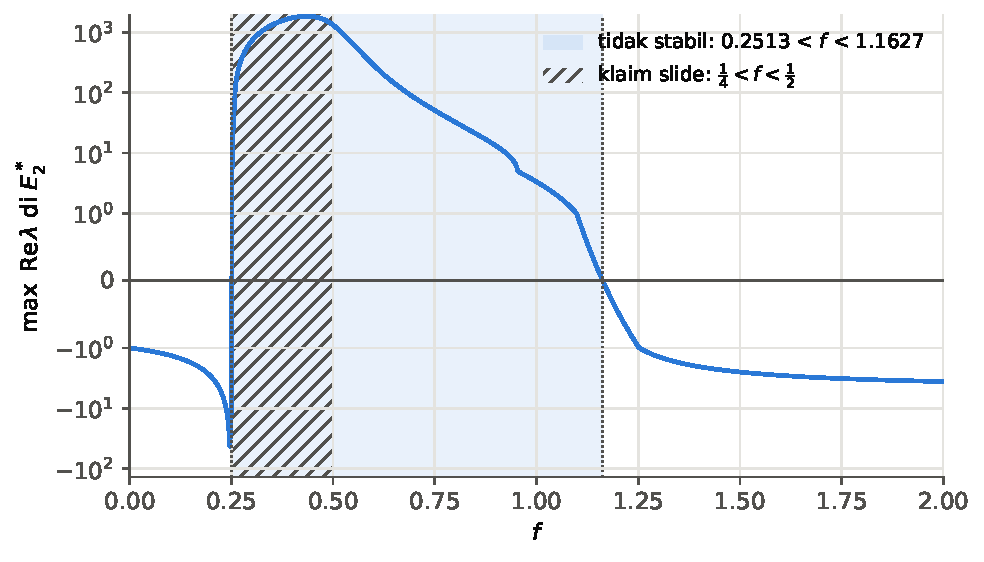
\includegraphics[width=\linewidth]{stability.pdf}
    \end{column}
    \end{columns}
\end{frame}

\subsection{Simulasi dan Interpretasi}

\begin{frame}{Simulasi dan Interpretasi}
    Simulasi ini akan menunjukkan pengaruh perubahan nilai parameter $f$ terhadap osilasi yang terjadi pada reaksi Belousov-Zhabotinsky.

    Dipilih nilai $\epsilon = 5 \times 10^{-5}$, $\delta = 2 \times 10^{-4}$, $q = 8 \times 10^{-4}$, dan nilai awal (tak berdimensi)
    $x_0 = 1.27 \times 10^{-7}$, $y_0 = 6 \times 10^{-7}$, $z_0 = 5 \times 10^{-3}$.
    Sistem bersifat \textit{stiff}, sehingga diintegrasikan dengan metode implisit (Radau, \texttt{rtol} $=10^{-9}$).
    \\
    Akan ditinjau beberapa nilai $f$:
\end{frame}

\begin{frame}{Simulasi dan Interpretasi}
    \begin{itemize}
    \item [1.]Untuk $f = 0.1$. Diperoleh grafik sebagai berikut:
    \begin{center}
        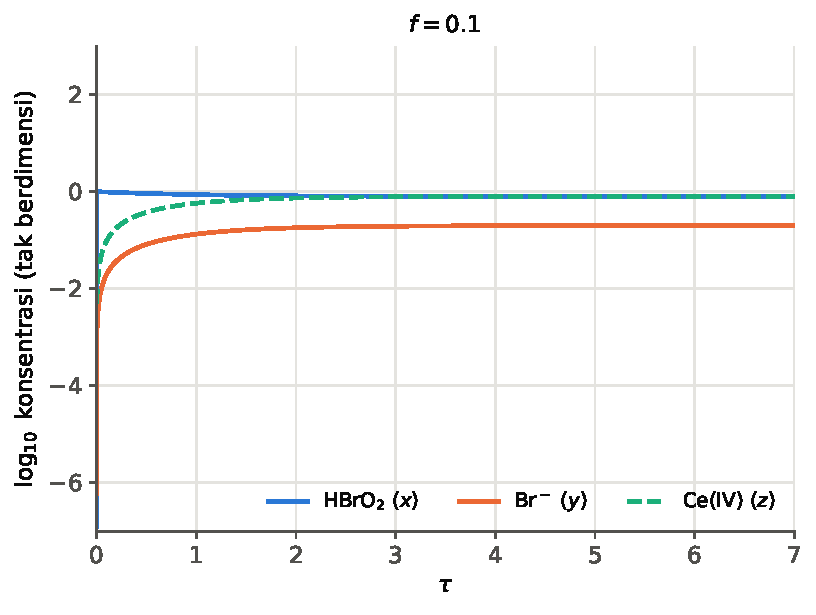
\includegraphics[height=0.68\textheight]{timeseries_f0.1.pdf}\\
        Gambar 2: Grafik $f = 0.1$
    \end{center}
    \end{itemize}
\end{frame}

\begin{frame}{Simulasi dan Interpretasi}
     Diperhatikan bahwa pada $f = 0.1$, solusi menuju titik kesetimbangan $E_{2}^{*} =  (0.800, 0.200, 0.800)$.
     Nilai ini tak berdimensi; konsentrasinya adalah $[HBrO_2] = X_0 x^*$, $[Br^{-}] = Y_0 y^*$, dan $[Ce(IV)] = Z_0 z^*$.
     Karena $f = 0.1 < 0.2513$, maka reaksi stabil sebagaimana yang dapat dilihat pada Gambar 2.
\end{frame}

\begin{frame}{Simulasi dan Interpretasi}
    \begin{itemize}
    \item [2.] Untuk $f = 0.4$. Diperoleh grafik sebagai berikut:
        \begin{center}
            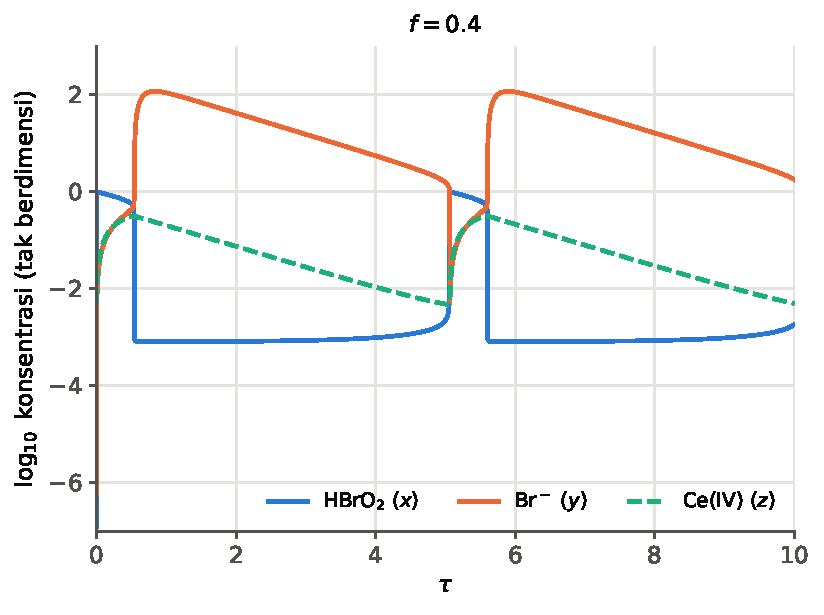
\includegraphics[height=0.68\textheight]{timeseries_f0.4.pdf}\\
            Gambar 3: Grafik $f = 0.4$
        \end{center}
    \end{itemize}
\end{frame}

\begin{frame}{Simulasi dan Interpretasi}
    Diperhatikan bahwa $0.2513 < f = 0.4 < 1.1627$ sehingga reaksi berosilasi. Periode osilasi yang diukur dari simulasi adalah
    $$T \approx 5.06$$
    dalam satuan $\tau$ (dalam detik, $t = T_0\,\tau$). Rumus linear $2\pi/\sqrt{C/A}$ hanya berlaku untuk osilasi kecil di dekat titik Hopf;
    di $f = 0.4$ osilasinya adalah osilasi relaksasi beramplitudo besar.

    \medskip
    Konsentrasi $HBrO_2$, $Ce(IV)$, dan $Br^{-}$ naik dan turun secara berulang – ulang dan sistem tidak kunjung setimbang. Naik turunnya konsentrasi $HBrO_2$, $Ce(IV)$, dan $Br^{-}$ ini dapat diamati sebagai munculnya perubahan warna yang membentuk suatu pola pada reaksi saat eksperimen dilakukan. Akibatnya, pada $f = 0.4$, sistem tidak stabil.
\end{frame}

\begin{frame}{Simulasi dan Interpretasi}
    \begin{columns}[T]
    \begin{column}{0.58\linewidth}
        \centering
        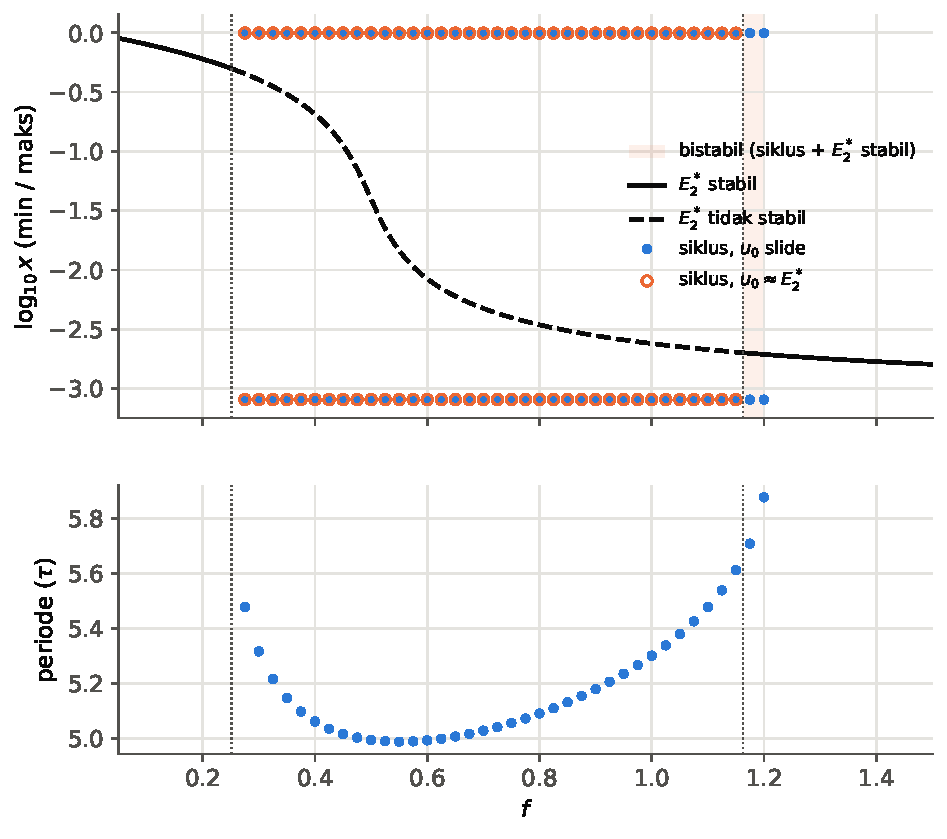
\includegraphics[height=0.8\textheight]{bifurcation.pdf}
    \end{column}
    \begin{column}{0.4\linewidth}
    \small
    Diagram bifurkasi: nilai minimum dan maksimum $\log_{10} x$ pada atraktor untuk setiap $f$.

    \medskip
    \begin{itemize}
        \item Osilasi muncul langsung dengan amplitudo besar setelah $f_{H,1} = 0.2513$.
        \item Untuk $1.1627 < f < 1.202$, siklus osilasi masih ada walaupun $E_2^*$ sudah stabil (bistabil): hasilnya bergantung pada nilai awal.
        \item Periode berada di kisaran 5--6 satuan $\tau$.
    \end{itemize}
    \end{column}
    \end{columns}
\end{frame}

\section{Kesimpulan}
\begin{frame}{Kesimpulan}
    \begin{itemize}
    \item [1.] Terdapat dua titik setimbang dari Model Sistem Dinamik Oregonator Reaksi Belousov - Zhabotinsky, yaitu $E_1^*=(0,0,0)$ dan $E_2^*=(x^*,y^*,z^*)$, di mana
        \begin{align}
        x^* = z^* = \tfrac{1-2f-q+\sqrt{(1-2f-q)^2+4q(1+2f)}}{2}, \qquad y^* = \tfrac{2fx^*}{q+x^*}. \notag
        \end{align}
     $E_2^*$ ada untuk setiap $f > 0$. Titik setimbang $E_1^*=(0,0,0)$ selalu tidak stabil dan titik setimbang $E_2^*=(x^*,y^*,z^*)$ mengalami bifurkasi.
     \item [2.] Bifurkasi pada titik setimbang $E_2^*$ adalah bifurkasi Hopf. Untuk parameter simulasi, $E_2^*$ tidak stabil dan sistem berosilasi apabila $0.2513 < f < 1.1627$. Osilasi juga dapat terjadi untuk $1.1627 < f < 1.202$, bergantung pada nilai awal.
     Batas atas $\tfrac12$ hanya diperoleh pada limit $q \to 0$.
     \item [3.] Osilasinya berupa osilasi relaksasi dengan periode sekitar 5 satuan $\tau$ ($T \approx 5.06$ pada $f = 0.4$).
     \end{itemize}
\end{frame}

\begin{frame}{Catatan Reproduksi (2026)}
    \small
    Analisis ini direproduksi ulang dengan Python (SymPy, SciPy).
    Perubahan terhadap versi Juni 2024:
    \begin{itemize}
        \item $\epsilon = k_0B/(k_5A)$, bukan kebalikannya; $q = 8\times10^{-6}$ dari konstanta laju.
        \item Rumus $x^*$, $y^*$ memakai $1-2f-q$ (bukan $1-f-q$); syarat $1-2f-q>0$ dihapus karena $E_2^*$ selalu ada.
        \item Koefisien $\lambda$ di $E_1^*$: $q(\epsilon-1)-\delta$, bukan $q(\epsilon+1)-\delta$.
        \item Interval ketidakstabilan $0.2513 < f < 1.1627$, bukan $\tfrac14 < f < \tfrac12$.
        \item Gambar 2 dan 3 dibuat ulang. Gambar asli ternyata hasil simulasi dengan $f \approx 5$ dan $f \approx 1$, bukan $0.1$ dan $0.4$.
        \item Periode di $f = 0.4$ adalah $T \approx 5.06$ (satuan $\tau$); nilai $6822.44$ tidak dapat direproduksi.
    \end{itemize}
    Kode dan rincian: \url{https://github.com/Peanut2Butter9/oregonator}
\end{frame}

\section{Referensi}

\begin{frame}{Referensi}
    \small
    A. M. Santoso, E. Apriliani, I G. N. R. Usadha, \emph{Analisis Kestabilan dan Bifurkasi Model Oregonator dari Reaksi Belousov – Zhabotinsky}, Jurnal Sains dan Seni ITS, Vol. 8, No. 1 (2019). doi:10.12962/j23373520.v8i1.42118

    \medskip
    R. J. Field, R. M. Noyes, \emph{Oscillations in chemical systems. IV. Limit cycle behavior in a model of a real chemical reaction}, J. Chem. Phys. 60, 1877 (1974).
\end{frame}

\begin{frame}
    \begin{center}
        {\Huge\calligra Terima kasih!}
    \end{center}
\end{frame}

\end{document}
